\documentclass[titlepage]{jsarticle}
\usepackage[dvipdfmx]{graphicx}
\usepackage{h31ec-exp}
\makeatletter
\newcommand{\figcaption}[1]{\def\@captype{figure}\caption{#1}}
\newcommand{\tblcaption}[1]{\def\@captype{table}\caption{#1}}
\makeatother
\title{光センサの使い方}
\grade{3年32番}
\author{平田 蓮}
\team{第10班}
\date{2019年7月22日}
\expdate{2019年7月1日,7月8日,7月22日}
\coauthor{
    8番 & 小林 歩夢 \\
    21番 & 相馬 拓杜 
}
\begin{document}
\maketitle
\section{目的}
    どのような制御システムでも, ~制御対象の減災の状態を知って次の適切な
    操作を決めるために, ~状態を計測するセンサが不可欠である. ~ここでは
    光センサの使い方について学ぶ.

    2種類の光センサを使用して, ~その特徴や基礎特性をまず理解しよう.
    ~次にセンサとして使用するための回路について検討し, ~その応用技術
    を身に付けよう.

\section{光センサの種類と選定}
    光センサと言っても様々な種類がある. ~例えば, ~フォトダイオード,
    ~フォトトランジスタ, ~光導電素子(CdSセル), ~焦電素子, ~光電管,
    ~カラーセンサ, ~個体イメージセンサ(CCD)などである. ~光センサの検出対象
    として, 「近赤外線, ~可視光線, ~紫外線といったどの波長を検出するのか?」
    また, 「どのような応答速度が必要なのか?」等の要因が重要になる.
    ~言い換えれば, ~検出対象の特性により, ~光センサの選定が必要となる.

\section{CdS光導電セル}
    \subsection{構造と原理}
        CdSセルは流下カドミウムを主成分とした光導電素子の一種であり,
        ~照射光によって内部抵抗が変化する一種の光抵抗器と考えることができる.

        図\ref{fig:CdS}にCdSセルの回路記号を示す. ~CdSセルは
        その性質上応答速度が非常に遅く, ~高速の光スイッチングには不向きである.
        ~その為, ~用途は緩やかな照度変化のセンシングに限定される. ~CdSセル
        には極性がなく, ~明るくなるとその内部抵抗は低下する.

        \begin{figure}[ht]
            \centering
            %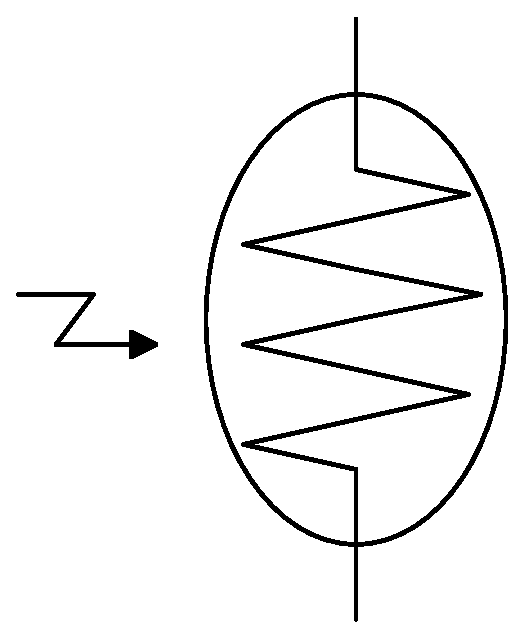
\includegraphics{images/CdS.eps}
            \caption{CdSセル回路記号}
            \label{fig:CdS}
        \end{figure}

    \subsection{基礎特性}
        光源にLEDを用いて, ~LEDの明るさによりCdSセルの抵抗値が変化
        することを確認しよう. ~なお, ~LEDに流れる電流と発光強度は正比例
        しないので, ~ここでは光の強度によりCdSセルの抵抗値が変化する
        ことを確認するための実験とする.

        \subsubsection{実験方法}
            \begin{enumerate}
                \item 図\ref{fig:kisotokusei}のように配線を行う.
                \item 電源電圧を0[V]から徐々にあげると電流$I_F$が
                    増加し, ~LEDの明るさが変化することと, ~CdSの
                    抵抗値$R_C$が変化していることを確認する.
                \item 電源電圧を変化させ, ~$I_F$が1[mA]から20[mA]
                    の時の$R_C$を測定しまとめる.
                \item 作成した表より, ~$I_F$-$R_C$グラフを両対数グラフ
                    で作成する.
            \end{enumerate}

            \begin{figure}[ht]
                \centering
                %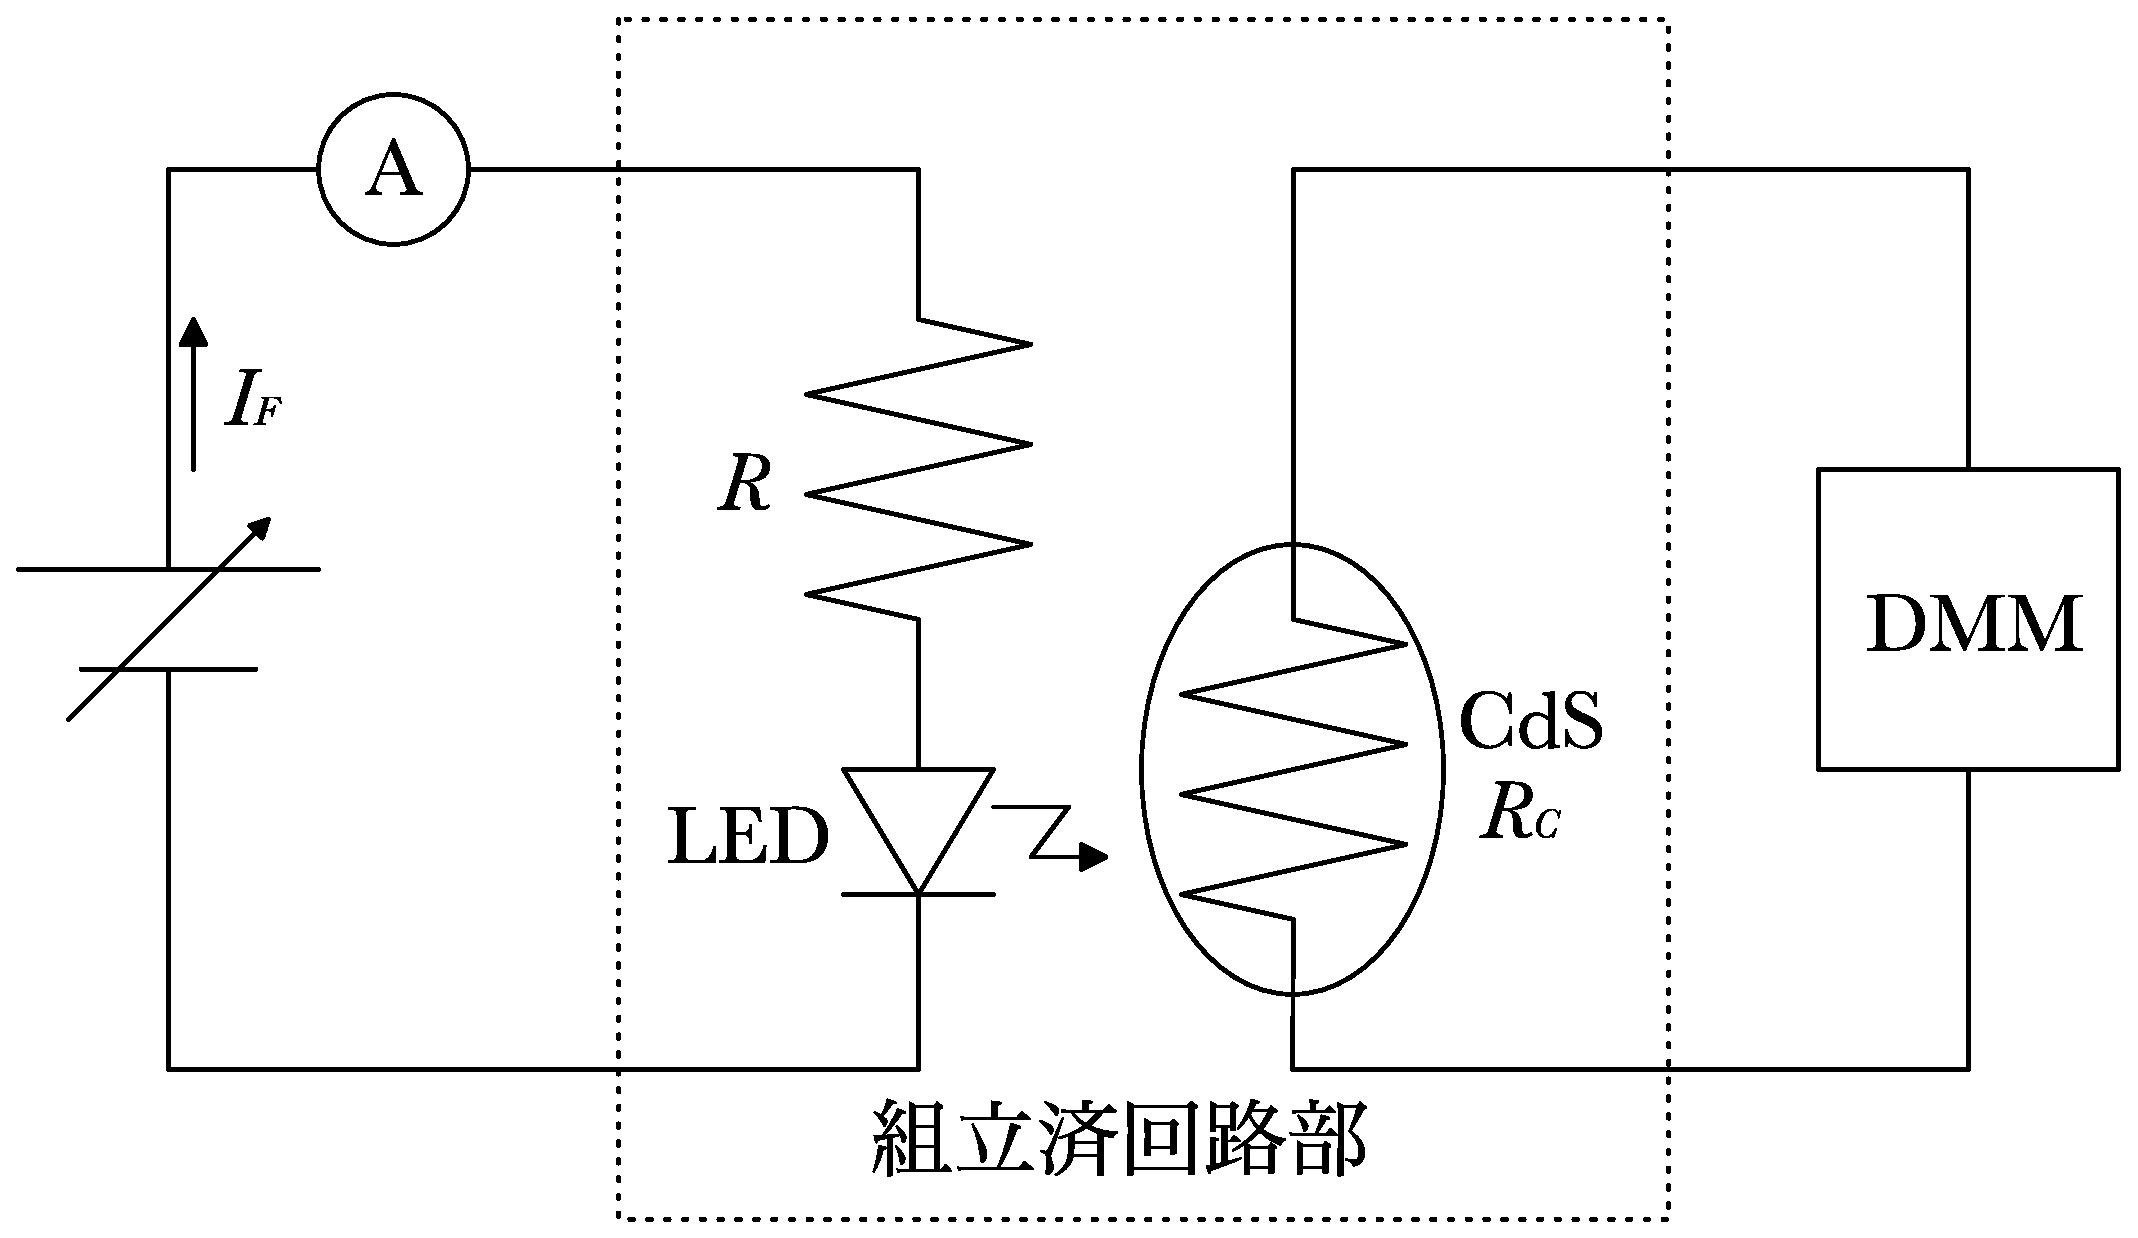
\includegraphics{images/CdS_circuit.eps}
                \caption{CdSセル基礎特性測定回路}
                \label{fig:kisotokusei}
            \end{figure}

        \subsubsection{使用素子 $\cdot$ 使用器具}
            \begin{description}
                \item[組み立て済み回路] CDS-A1
                \item[CdSセル] MKY-54C348
                \item[LED] L-513SGT3
                \item[デジタルマルチメータ] EC-12
                \item[直流電源] Ec-01
                \item[電流計] 341 
            \end{description}

        \subsubsection{結果}
            図\ref{tab:kisotokuseikekka}, \ref{fig:kisotokuseigraph}
            に結果の表とグラフを示す.

            \begin{figure}[ht]
                \def\@captype{table}
                \begin{minipage}{0.5\hsize}
                    \begin{center}
                        \caption{基礎特性測定結果}
                        \label{tab:kisotokuseikekka}
                        \begin{tabular}{c|c}
                            
                        \end{tabular}
                    \end{center}
                \end{minipage}
                \begin{minipage}{0.5\hsize}
                    \begin{center}
                        %\includegraphics[width=8cm]{graphs/kisotokusei.pdf}
                        \caption{基礎特性グラフ(両対数)}
                        \label{fig:kisotokuseigraph}
                    \end{center}
                \end{minipage}
            \end{figure}

    \subsection{明暗判定回路}
        CdSセルを用いて, ~暗くなったら赤色LEDを点灯させる簡単な回路を
        作成してみよう.

        \subsubsection{実験方法}
            \begin{enumerate}
                \item 図\ref{fig:hanteikairo}のように配線を行う.
                    ~$VR$は10[k$\Omega$]の半固定抵抗とし,
                    ~$R$は1[k$\Omega$]の炭素皮膜抵抗とする.
                    ~また, ICには5[V]の電源電圧を供給する.
                \item CdSセルに蛍光灯の光が当たっている場合には
                    LEDが消灯し, ~CdSに当たっている光が遮断された
                    場合にはLEDが点灯するように$VR$を調節する.
            \end{enumerate}

            \begin{figure}[ht]
                \centering
                %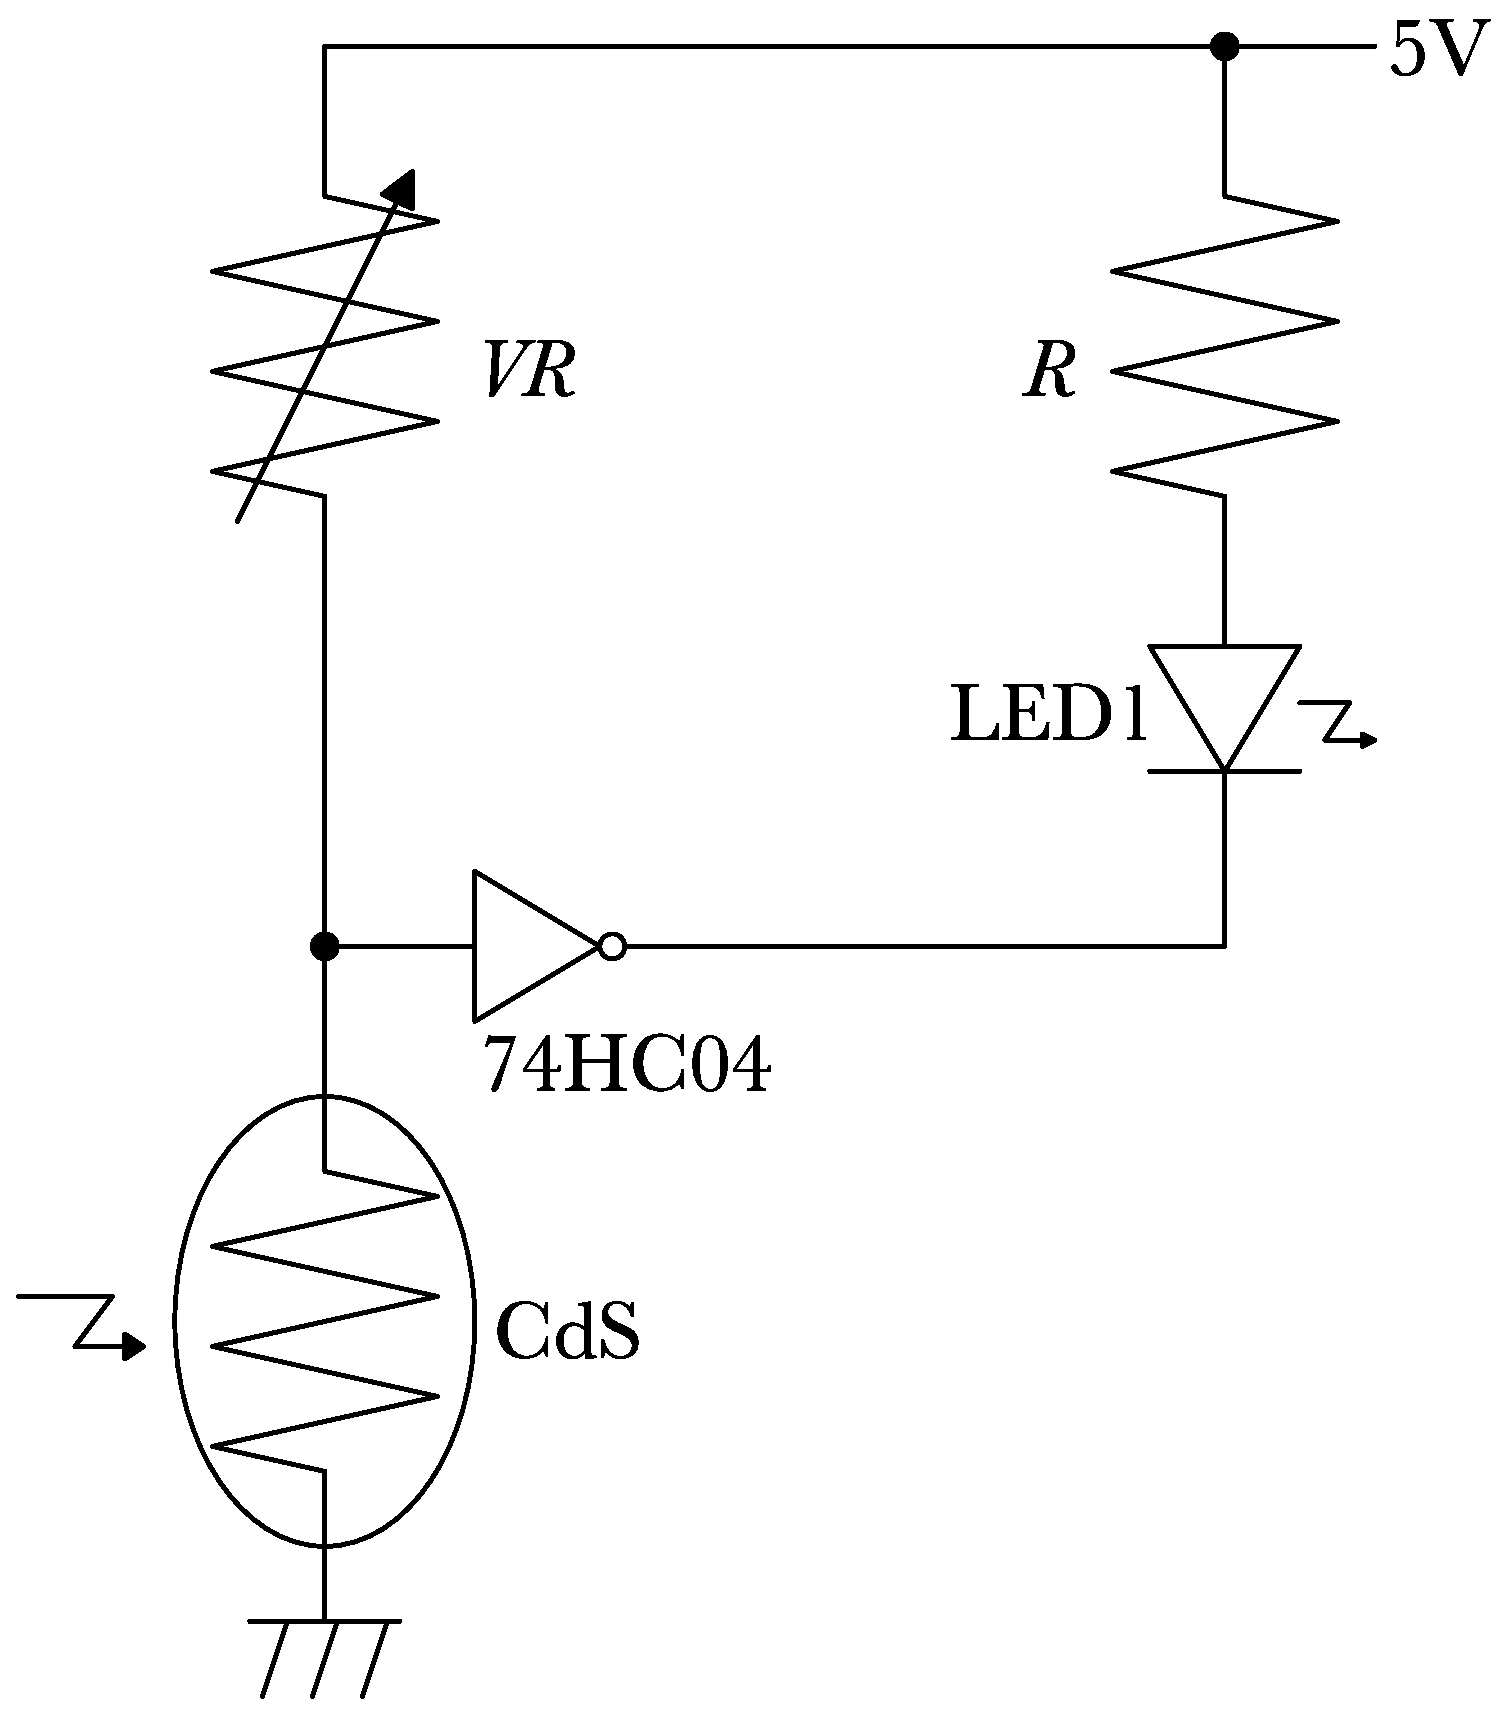
\includegraphics{images/hanteikairo.eps}
                \caption{明暗判定回路}
                \label{fig:hanteikairo}
            \end{figure}

        \subsubsection{使用素子 $\cdot$ 使用器具}
            \begin{description}
                \item[CdSセル] MKY-54C348
                \item[LED] L-513LE1T
                \item[IC] 74HC04
                \item[デジタルマルチメータ] EC-12
                \item[直流電源] Ec-01
                \item[ブレッドボード] EC-16 
            \end{description}

        \subsubsection{結果 $\cdot$ 考察}
            CdSセルに指をかざすとLEDが点灯し, ~指を離すと再び点灯した.

            これは, ~光が遮断されることでCdSの抵抗値が増え, ~C点での
            電圧が高くなり, ~NOTを通したB点の電圧が低くなり, ~A-B間に
            電位差が生まれるためである.

    \subsection{応用回路}

\section{フォトダイオード}
    \subsection{構造と原理}

    \subsection{短絡特性}
        \subsubsection{実験方法}

        \subsubsection{結果}

    \subsection{開放特性}
        \subsubsection{実験方法}

        \subsubsection{結果}

    \subsection{照度計}

    \subsection{蛍光灯の光観察}
        \subsubsection{実験方法}

        \subsubsection{結果}

\end{document}
